%
% File acl2021.tex
%
%% Based on the style files for EMNLP 2020, which were
%% Based on the style files for ACL 2020, which were
%% Based on the style files for ACL 2018, NAACL 2018/19, which were
%% Based on the style files for ACL-2015, with some improvements
%%  taken from the NAACL-2016 style
%% Based on the style files for ACL-2014, which were, in turn,
%% based on ACL-2013, ACL-2012, ACL-2011, ACL-2010, ACL-IJCNLP-2009,
%% EACL-2009, IJCNLP-2008...
%% Based on the style files for EACL 2006 by 
%%e.agirre@ehu.es or Sergi.Balari@uab.es
%% and that of ACL 08 by Joakim Nivre and Noah Smith

\documentclass[11pt,a4paper]{article}
\usepackage[hyperref]{acl2021}
\usepackage{times}
\usepackage{latexsym}
\renewcommand{\UrlFont}{\ttfamily\small}

% This is not strictly necessary, and may be commented out,
% but it will improve the layout of the manuscript,
% and will typically save some space.
\usepackage{microtype}

% \aclfinalcopy % Uncomment this line for the final submission
%\def\aclpaperid{***} %  Enter the acl Paper ID here

%\setlength\titlebox{5cm}
% You can expand the titlebox if you need extra space
% to show all the authors. Please do not make the titlebox
% smaller than 5cm (the original size); we will check this
% in the camera-ready version and ask you to change it back.

\newcommand\BibTeX{B\textsc{ib}\TeX}

\title{Integrating Word Knowledge and WordNet for Neural Metaphor Detection}
% \title{Knowledge Integration for Neural Metaphor Detection}

\author{First Author \\
  Affiliation / Address line 1 \\
  Affiliation / Address line 2 \\
  Affiliation / Address line 3 \\
  \texttt{email@domain} \\\And
  Second Author \\
  Affiliation / Address line 1 \\
  Affiliation / Address line 2 \\
  Affiliation / Address line 3 \\
  \texttt{email@domain} \\}

\date{}

\begin{document}
\maketitle
\begin{abstract}
   The ubiquity of metaphor in daily life results metaphor detection a crucial part for many natural language processing tasks. We believe that the knowledge is crucial to detect the metaphor. An effective end-to-end metaphor detection framework which concatenates transformer model with knowledge integration and WordNet graph embedding is proposed. Besides, some additional word attributes in the word embedding layer are added to further increase the performance of the model. The experimental results on two popular datasets shows that our model outperforming the current state-of-the-art models.

\end{abstract}

% \section{Credits}

% This document has been adapted by Roberto Navigli
% from the instructions for earlier ACL, NAACL and EMNLP proceedings, including those for 
% EMNLP 2020 by Yulan He,
% ACL 2020 by Steven Bethard, Ryan Cotterrell and Rui Yan, 
% ACL 2019 by Douwe Kiela and Ivan Vuli\'{c},
% NAACL 2019 by Stephanie Lukin and Alla Roskovskaya, 
% ACL 2018 by Shay Cohen, Kevin Gimpel, and Wei Lu, 
% NAACL 2018 by Margaret Michell and Stephanie Lukin,
% 2017/2018 (NA)ACL bibtex suggestions from Jason Eisner,
% ACL 2017 by Dan Gildea and Min-Yen Kan, 
% NAACL 2017 by Margaret Mitchell, 
% ACL 2012 by Maggie Li and Michael White, 
% ACL 2010 by Jing-Shing Chang and Philipp Koehn, 
% ACL 2008 by Johanna D. Moore, Simone Teufel, James Allan, and Sadaoki Furui, 
% ACL 2005 by Hwee Tou Ng and Kemal Oflazer, 
% ACL 2002 by Eugene Charniak and Dekang Lin, 
% and earlier ACL and EACL formats written by several people, including
% John Chen, Henry S. Thompson and Donald Walker.
% Additional elements were taken from the formatting instructions of the \emph{International Joint Conference on Artificial Intelligence} and the \emph{Conference on Computer Vision and Pattern Recognition}.

\section{Introduction}

Metaphor expressions appear pervasively in daily life as well as in many literary works. It is estimated to occur once in every three sentences on average \cite{bilsky1952ia}. People use metaphor frequently because metaphor expression may furnish vivid explanations for experience and perception. Metaphors can be understood as a systematic mapping from a concrete conceptual source domain to an abstract target domain \cite{1982Lakoff}. For instance, the metaphorical sentence “She devoured his novels” utilizes the verb “devour” to convey a sense of greedy reading rather than literally swallowing a novel. The ubiquity of metaphor gives rise to the difficulty of language understanding in natural language processing. While lots of research has been done to understand the metaphor, most methods can be divided into two steps: (1) metaphor detection and (2) metaphor interpretation. This paper focuses on the first step: metaphor detection. 

Most latest successful metaphor detection methods exploit neural network methods by incorporating word embedding, context, semantic information. Observing that one is likely to have a higher performance on metaphor detection if he has more knowledge about an event, this paper tries to integrate knowledge during detecting metaphor. In particular, we propose a novel framework to incorporate word knowledge information, such as POS, TAG, definition, and WordNet Graph Embedding. The experimental results on two popular datasets shows that integrating word knowledge can be very useful to detect metaphors.

The contribution of this paper includes: (1) Prove that augmenting word’s knowledge and incorporating knowledge base is able to improve the performance of metaphor detection. (2) Propose a novel metaphor detection framework to effectively integrating the knowledge. (3) Run extensive experiments on two metaphor detection datasets and outperforming the current state-of-the-art models.



\section{Related Work}
\subsection{Metaphor Detection}
Early research on computational metaphors identification was based on statistical features, such as unigrams \cite{beigman-klebanov-etal-2014-different}, bag-of-words features \cite{koper-schulte-im-walde-2016-distinguishing}, concreteness, abstractness \cite{tsvetkov2014metaphor}, With a recent surge of interest in neural networks, Some studies combined feature in supervised machine learning \cite{turney-etal-2011-literal,beigman-klebanov-etal-2016-semantic}, deep learning \cite{rei-etal-2017-grasping,gutierrez-etal-2017-using} and unsupervised learning \cite{shutova-2015-design,mao2018word} approaches.
Recently, metaphor identification has been treated as a sequential labeling task. \citet{wu2018neural} established the pre-trained word vector for input and then used the combination of CNN and BiLSTM for processing. \citet{mao2019end} applied linguistic theory to improve the performance of the model. \citet{rohanian-etal-2020-verbal} found that there is an overlap between metaphor identification and Multi-Word Expression (MWE), combining graph convolutional networks and BERT \cite{devlin2018bert} to achieve the state-of-the-art on MOH-X and TroFi dataset.
\subsection{Task Transferring}
\citet{mccann2018natural} showed that converting NLP tasks into question-answering tasks can significantly improve the model's performance. Many NLP tasks can be converted into question-answering tasks, such as sentiment analysis tasks, which can be converted into asking the machine whether it is positive for a given sentence. This transformation has achieved good results in some tasks. Some studies also tried to solve NER (Named Entity Recognization) tasks by converting the model into question-answering tasks \cite{li2019unified}.

\subsection{Graph Embedding}
 Graph embedding means that a low-dimensional, dense vector represents the points in the graph. Unlike other studies that use WordNet directly, we use the embedding of a word in WordNet. Training a graph embed requires many computing resources, we use the pre-trained WordNet Embedding \cite{saedi2018wordnet}.


\section{Knowledge Integration Neural Metaphor Detection Model}

\begin{figure*}[htbp]
    \centering
    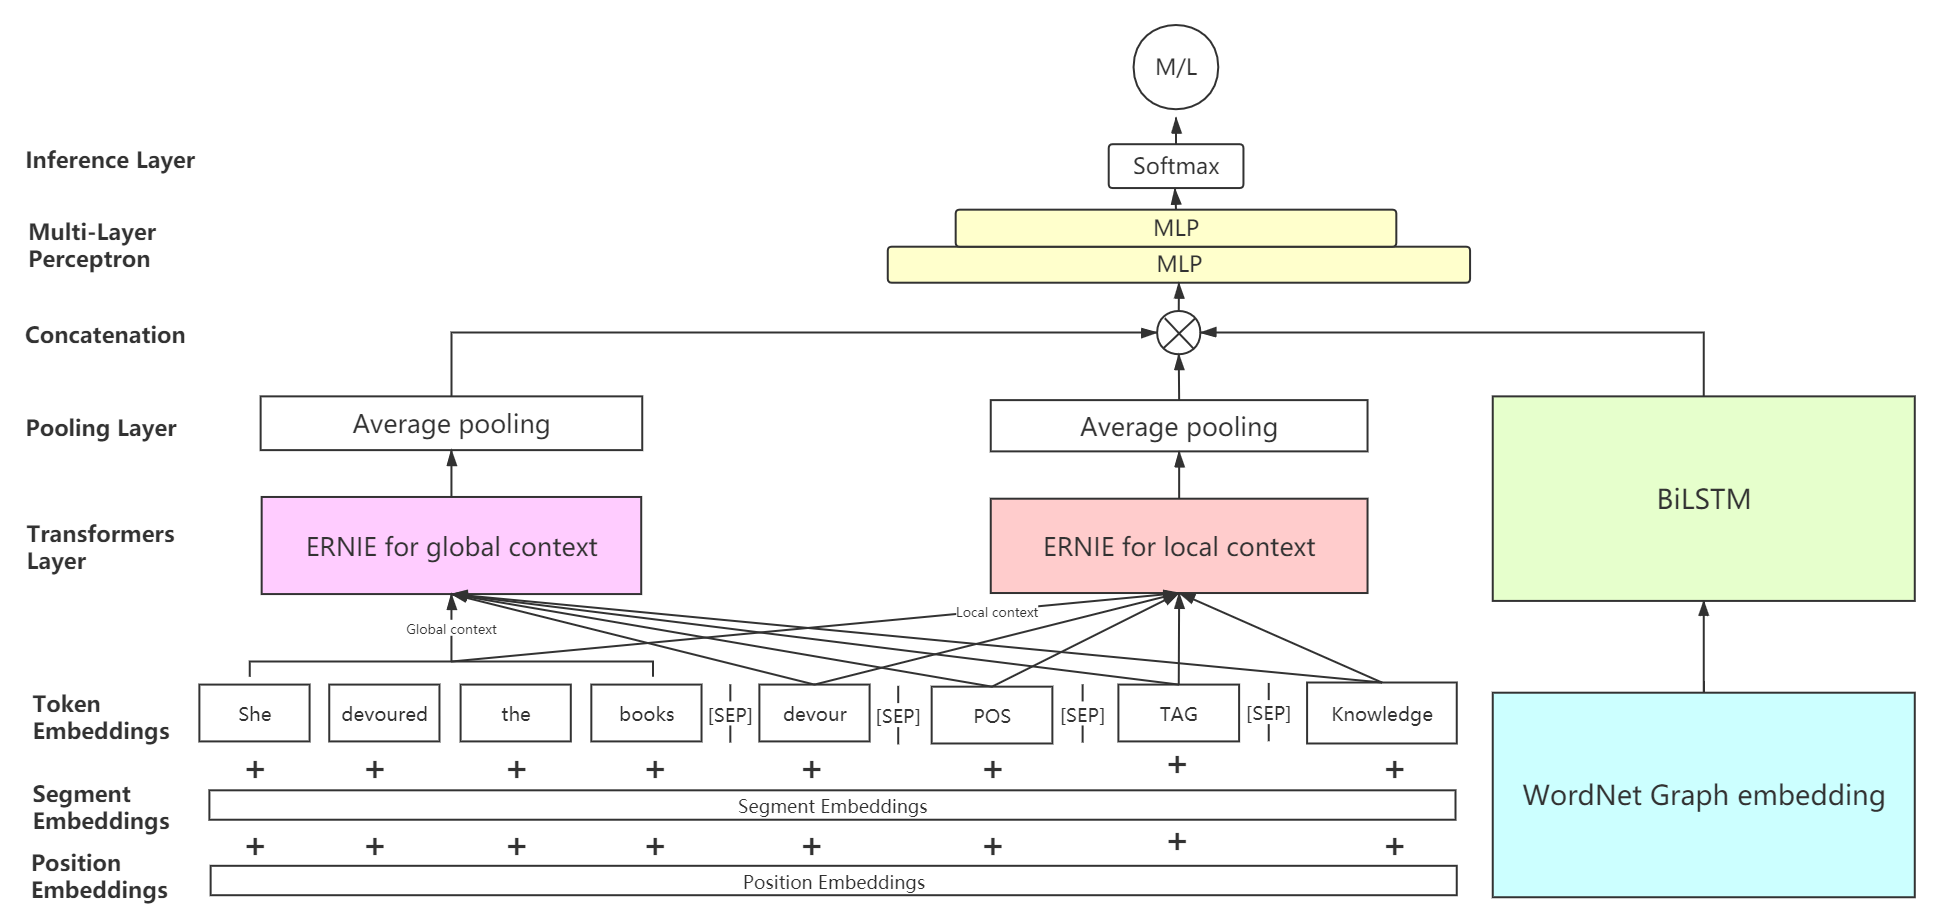
\includegraphics[scale=0.22]{asset/model2.png}
    \caption{Model structure of Knowledge Integration for Neural Metaphor Detection. The model combines context, query word, POS, TAG and knowledge as token embedding. Use token embedding, segment embedding and position embedding as the input of two transformer models: ERNIE for capturing global context and another ERNIE for local context. The output of transformer models are processed by average pooling layer and concatenate with BiLSTM on WordNet Graph Embedding. The concatenation result processes through two layers of MLP and use Softmax to calculate the probability.}
    \label{img1}
\end{figure*}

Knowledge Integration Neural Metaphor Detection Model (shown in Figure \ref{img1}) incorporates different information of specific words, including POS, TAG, and definition to the embedding layer. Two separate pre-trained transformer Enhanced Representation through knowledge Integration (ERNIE 2.0) \cite{sun2020ernie} units are constructed to handle the global and local contexts. Afterwards, we concatenate the hidden layer output of the ERNIE units and bidirectional long short-term memory (BiLSTM) output of the WordNet Graph embedding with two layers of MLP (Multi-Layer Perception). 

% In this section, we describe (1) our enhanced word embedding on how we includes more information in the transformer embedding layer (2) our knowledge integration strategy on how we use ERNIE and WordNet Graph Embedding with BiLSTM.

\subsection{Enhanced Embedding Layer}
Inspired by \citet{mccann2018natural}, we transfer the metaphor detection sequence labeling task into a question-answering task. We do not merely give the context, question, and answer. Each word's additional information is provided, including POS (Part Of Speech), TAG (Detail information of POS), and knowledge. With this kind of augmentation, given the word extra information to answer a specific question may perform better than solely provide the context information. 
For instance, the question-answering task becomes: \\
(1) Given the context ``She devoured the book."\\
(2) Enriched with the information of the word ``devoured" with knowledge ``destroy completely; enjoy avidly, eat up completely", and ``devoured" is a verb with past tense.\\
(3) Ask the word "devoured" with the above information if it is ``metaphorical" or ``literal".

For each word's POS and TAG, we utilize the toolkit Stanza \cite{qi2020stanza}, which is the Stanford NLP Group's official Python NLP library. POS means Part of Speech, which would judge a word what sort of part of speech given the belonging sentence. For TAG means Detail of Part of Speech, includes a more comprehensive classification on terms. For instance, consider the sentence ``Barack Obama was born in Hawaii." The word ``born" would be labeled as VERB in POS and would be labeled as VBN in TAG, which means ``Type: Past Verb, VerbForm: Part". For each query word's knowledge, which is the definition of words, we utilize the NLTK (Natural Language Toolkit) tool connecting to WordNet and search for specific word definition. Therefore, we concatenate the context, word to be queried, POS, TAG, knowledge of word and answer of metaphorical or literal together for enhanced embedding layer.

% We use the transformer embedding layer to represent our input sequence. 
% $[CLS]$ is used at the first token as special classification $[SEP]$ is used for separating sentences, here we used as separating different features, and $[UNK]$ is added for an unknown token, especially useful when we cannot find the knowledge information. Therefore, the entire embedding would be token embedding, segment embedding, and position embedding.

\subsection{Knowledge Integration Strategy}
After enhanced embedding, the embedding should transfer to fit the transformer. The transformer word embedding includes the token embedding, segment embedding, and position embedding. Those embedding are fed into a double parallel transformer encoder model—processing both global and local context for the metaphor detection task. WordNet Graph Embedding with BiLSTM is also concatenated for further processing. The reason for concatenating two parts is that we hope our model can process through combining the context meaning with existed knowledge and word meaning with online knowledge base by WordNet Graph Embedding.


ERNIE 2.0 \cite{sun2020ernie} is a continual pretraining transformer framework specializing in extracting the lexical, syntactic, and semantic information by augmenting knowledge training. The transformer module is composed of multi-head self-attention encoders. The formulas are shown as  below:

\begin{small}
$$ R^i = Softmax(\frac{QK^T}{\sqrt{d}})\eqno{(1)} $$
$$ Attention-output =Att(Q, K, V) = R^iV^i \eqno{(2)}$$
$$ head_i = Att(QW_i^Q, KW_i^K, VW_i^V) \eqno{(3)}$$
$$ MultiHead(Q, K, V) = Concat(\sum_{i=1}^h(head_i))W^0 \eqno{(4)}$$
\end{small}

$Q$, $K$, and $V$ are respectively query matrix, key matrix and value matrix, $i$ indicates the index of self-attention. $d$ is the scaling parameter. $W^Q$, $W^K$, and $W^V$ are the weights of the self-attention module. Function $Concat$ means the concatenation of tensors. Function $Att$ means the attention mechanism. The entire encoder module first deals with the Multi-head Self Attention mechanism then feeds through ``Add \& Norm" for Batch Normalization, then comes to feedforward networks and does the Batch Normalization again for processing.
\makeatletter\def\@captype{table}\makeatother
\begin{table*}[!htbp] 
\centering
\begin{tabular}{lllllllllll|llllllllllll|llllllllllll|llllllllllll}
% \begin{center}

\hline
\multicolumn{11}{l|}{{Model}} & \multicolumn{12}{c|}{{VUA VERB}}  & \multicolumn{12}{c|}{{VUA ALL POS}} & \multicolumn{12}{c}{{MOH-X}} \\
\multicolumn{11}{l|}{{\quad}}   &\multicolumn{4}{c}{{P}} & \multicolumn{4}{c}{{R}} & \multicolumn{4}{c|}{{F1}}  & \multicolumn{4}{c}{{P}} & \multicolumn{4}{c}{{R}} & \multicolumn{4}{c|}{{F1}} &\multicolumn{4}{c}{{P}} & \multicolumn{4}{c}{{R}} & \multicolumn{4}{c}{{F1}} \\ \hline
\multicolumn{11}{l|}{\citet{gao2018neural}} &\multicolumn{4}{c}{{53.4}} & \multicolumn{4}{c}{{65.6}} & \multicolumn{4}{c|}{{58.9}}  &\multicolumn{4}{c}{{68.2}} & \multicolumn{4}{c}{{71.3}} & \multicolumn{4}{c|}{{69.7}}   &\multicolumn{4}{c}{{75.3}} & \multicolumn{4}{c}{{84.3}} & \multicolumn{4}{c}{{79.1}} \\
\multicolumn{11}{l|}{RNN-HG} &\multicolumn{4}{c}{{69.3}} & \multicolumn{4}{c}{{72.3}} & \multicolumn{4}{c|}{{70.8}}  &\multicolumn{4}{c}{{71.8}} &\multicolumn{4}{c}{{76.3}} & \multicolumn{4}{c|}{{74.0}}   &\multicolumn{4}{c}{{79.7}} & \multicolumn{4}{c}{{79.8}} & \multicolumn{4}{c}{{79.8}}\\
\multicolumn{11}{l|}{RNN-MHCA}  &\multicolumn{4}{c}{{66.3}} & \multicolumn{4}{c}{\textbf{75.2}} & \multicolumn{4}{c|}{{70.5}}  &\multicolumn{4}{c}{\textbf{73.0}} &\multicolumn{4}{c}{{75.7}} & \multicolumn{4}{c|}{\textbf{74.3}}    &\multicolumn{4}{c}{{77.5}} & \multicolumn{4}{c}{{ 83.1}} & \multicolumn{4}{c}{{ 80.0}}\\ 
\multicolumn{11}{l|}{BERT+MWE-Aware GCN}   &\multicolumn{4}{c}{{-}} &\multicolumn{4}{c}{{-}} & \multicolumn{4}{c|}{{-}}   &\multicolumn{4}{c}{{-}} & \multicolumn{4}{c}{{-}} & \multicolumn{4}{c|}{{-}}&\multicolumn{4}{c}{{79.98}} & \multicolumn{4}{c}{{80.40}} & \multicolumn{4}{c}{{80.19}}\\ \hline
\multicolumn{11}{l|}{ERNIE+WordNet} &\multicolumn{4}{c}{\textbf{78.19}} & \multicolumn{4}{c}{{73.71}} & \multicolumn{4}{c|}{\textbf{75.88}}  &\multicolumn{4}{c}{{66.84}} &\multicolumn{4}{c}{\textbf{78.91}} & \multicolumn{4}{c|}{{72.37}}    &\multicolumn{4}{c}{\textbf{89.02 }} & \multicolumn{4}{c}{\textbf{ 96.05}} & \multicolumn{4}{c}{\textbf{ 92.41}}
% \end{center}
\end{tabular}
\caption{Experimental result of different models on VUA and MOH-X datasets}
\label{table1}
\end{table*}

Two ERNIE units play different roles: one ERNIE unit encodes global context and another unit encodes local context. Their output is sent into the average pooling to reduce the dimension and obtain the generalized metaphor features. The output after pooling are concatenated together with the 850 dimensions WordNet Graph Embedding processing with the BiLSTM layer. The training procedure of WordNet Graph Embedding is based on the length and number of the connection between two words in WordNet. The results show that WordNet graph embedding performance is higher than Word2Vec in some Semantic Similarity Tasks. The embedding is training on Princeton WordNet \cite{fellbaum1998wordnet} which contain over 25 types of semantic relations and over 155k words (lemmas). The concatenated output is processed to 2 layers of Multi-Layer Perception (MLP) with 1024 dimensions. In the end, the model predicts the probability through an inference layer with a $Softmax$ function. 

$$V = Concat(E_1, E_2, N_1) \eqno{(5)}$$
$$ W_t, b = MLP(V) \eqno{(6)}$$
$$ y_t = Softmax(W_t+b) \eqno{(7)}$$

$E_1$ and $E_2$ respectively indicate the ERNIE transformer's hidden layer output for Global Context and ERNIE transformer for Local Context. $N_1$ indicates the output vector of BiLSTM with WordNet Graph Embedding. $W_t$ and $b$ are the output parameters matrix of 2 layers of MLP, and $y_t$ is the output probability of metaphorical and literal words. 

Cross-entropy is used as the cost function. The probability output is set with a variety of thresholds to judge if the word is metaphorical or literal.

% \subsection{Fully-connected Layer and Loss Function}

% The model is training through a cross-entropy loss function $L$, which is shown below:

% \begin{small}
% $$ L_{verb} = L_{AllPOS} = - \sum{i=1}^{M}(ylogy_L+(1-y)logy_m) $$
% \end{small}


% $y$ is the label of ground truth, $L_{verb}$ is the loss value of verb, and $L_{AllPOS}$ is the loss value of all the POS.In the inference layer, we use cross-entropy as the cost function, and We introduce the Dropout mechanism to prevent over-fitting and the Adam optimizer for random improvement during training during the t

\section{Experimental Result}
\subsection{Dataset}
Two widely used datasets: VU Amsterdam Metaphor Corpus (VUA) and MOH-X are used in the experiments.

VUA (VU Amsterdam Metaphor Corpus) is the largest manually labeled figurative language Corpus among various fields published in the metaphor detection task \cite{krennmayr2017vu}. It consists of four categories of texts: academic texts, novel texts, news texts, and dialogue texts. The language contains more than 2626 paragraphs, 16,000 sentences, and about 200,000 words. VUA dataset contains relatively long sentences.

MOH-X corpus \cite{mohammad2016metaphor} is a subset of the MOH corpus. The corpus texts are all from the WordNet with annotated for metaphorical verbs along with associated confidence scores. Only a single target verb in each sentence is labeled. Sentences in relatively short. This dataset has 214 unique verbs.

\subsection{Experiments}

Besides our model, a number of state-of-the-art neural network-based metaphor detection models have also implemented:\\
(1)\citet{gao2018neural}: This model utilizes GloVe+ELMo for word embedding and BiLSTM as an encoder.\\
(2) RNN-HG and RNN-MHCA \cite{mao2019end}: These models utilize the BiLSTM+attention mechanism for implementation on two linguistic theories Selectional Preference Violation and Metaphor Identification Procedure, respectively.\\
(3) BERT+MWE-Aware GCN \cite{rohanian-etal-2020-verbal}: A metaphor detection model published on ACL2020 with BERT as encoder and Graph Convolution Network for processing multi-word expressions. \\
The evaluation metrics include precision (P), recall (R), and F1-score (F1). According to the result, our model has some significant improvement (shown in Table \ref{table1}): the results show our model reaches 75.88\% F1 score on the VUA verb test set and 92.41\% on the MOH-X dataset, outperforming other state-of-the-art metaphor detection model. For MOH-X, We slightly modify our model from two ERNIE modules to one since the MOH-X dataset contains almost short sentences.
\\

\section{Conclusion}
We propose a novel metaphor detection framework. Our model incorporates transformers with knowledge integration and WordNet knowledge base into the neural network model. The experiments show that knowledge integration is a powerful tool of metaphor detection.


\bibliographystyle{acl_natbib}
\bibliography{acl2021}

%\appendix



\end{document}
